\documentclass[a4paper]{article}
\usepackage{fullpage}
\usepackage{amsfonts} % pour les lettres maths creuses \mathbb
\usepackage{amsmath}
\usepackage[T1]{fontenc}
\usepackage[utf8]{inputenc}
\usepackage[frenchb]{babel}
\usepackage{aeguill}
\usepackage{graphicx}
\usepackage{hyperref}
\usepackage{color}
\usepackage{listings}
\usepackage{pdfpages}
% Another method to track changes
% Examples of usage:
% - This is \added[id=per,remark={we need this}]{new} text.
% - This is \deleted[id=per,remark=obsolete]{unnecessary}text.
% - This is \replaced[id=per]{nice}{bad} text.
% To print the list of change use: \listofchanges
%~ \usepackage{changes}	% use this for the working version
%\usepackage[final]{changes} % use this for the final version
%~ \definechangesauthor[name={Andrea Del Prete}, color=orange]{adp}
\newcommand{\deladp}[1]{\textcolor{red}{#1}}
\newcommand{\addadp}[1]{\textcolor{green}{#1}}
%~ \newcommand{\repadp}[2]{\replaced[id=adp]{#1}{#2}}
%~ \definechangesauthor[name={Steve Tonneau}, color=blue]{st}
%~ \newcommand{\delst}[1]{\deleted[id=st]{#1}}
%~ \newcommand{\addst}[1]{\added[id=st]{#1}}
%~ \newcommand{\repst}[2]{\replaced[id=st]{#1}{#2}}
\newcommand{\gls}[1]{\textit{#1}}
\newcommand{\glslink}[2]{{#2}}
%~ \newcommand{\done}[0]{\textcolor{green}{DONE}}
\newcommand{\done}[0]{}
\newcommand{\ndone}[0]{\textcolor{red}{TODO}}

\newcommand\dx{\dot{x}}
\newcommand\dy{\dot{y}}
\newcommand\ddx{\ddot{x}}
\newcommand\ddy{\ddot{y}}
\def\real{{\mathbb R} }
\newcommand\quot[1]{\begin{quote} \underline{quote}: \textbf{#1}\end{quote}}
\newcommand\as[1]{\begin{quote} \underline{answer}: {#1}\end{quote} }
\newcommand\qt[1]{\begin{quote} \underline{added text in paper}: \textit{#1}\end{quote} \leavevmode \\ }
\newcommand\jp{ \leavevmode \\}
\frenchbsetup%
{%
StandardItemLabels=true,%
ItemLabels=\ding{43},%
}%
\DeclareUnicodeCharacter{00A0}{ }
\author {}
\title {Cover letter for the resubmission of our paper ``An efficient acyclic contact planner for multiped robots''}
\date {}

%% \addtolength{\oddsidemargin}{-.6in}
%% \linespread{1.5}
%% \addtolength{\textwidth}{-1.5in}

\begin{document}
\maketitle

\section{Summary of the modifications}

First of all, we would like to thank all the reviewers and the associate editor (AE).
We received three detailed and technical reviews that helped improving our paper.
Overall we agreed with most of the reviews and took them into account in the revised version of the paper.
The main points of concern raised by the reviewers regarded:
\begin{itemize}
\item the diffficulty to understand the takeaway message of the paper, and what was novel with respect to our previous paper [20] (and [1] to a lesser extent);
\item the organization of the paper, with too much information relegated to the Appendix, or only referred to in other contributions.
\end{itemize}

\textbf{Regarding the contribution of this paper with respect to our previous papers}, this paper must be understood
as an extension of [20] (presented at the ISRR conference). As a self-contained journal paper, the present paper aims at replacing [20]. We present two contributions. The first one, as in [20], is an efficient and generic planning method for multi-contact locomotion (problems P1 and P2).
The second one is a rigorous experimental validation of the approach on actual robot models, either in simulation or on the real HRP-2 robot.

Regarding the first contribution, the algorithm presented here is the same as in [20], but with three important novelties: a novel criterion for
static equilibrium, the pseudo-code of the algorithm,
as well as  the release of the source code of the planner.

Regarding the second contribution, to validate the contact plans computed we introduced a complete framework for multi-contact motion synthesis. This framework additionally comprises an interpolation method to solve the problem P3, similar but not identical to the one we proposed in [1]. It also comprises an implementation of a state-of-the-art dynamic simulator to check that the motions are physically plausible [28]. These aspects of the framework are presented in details in the paper, but are not novel \textit{per se}. The novelty lies in the validation of the method with real robot models, for which the planning is harder with respect to the avatars used in [20], because of stricter kinematic constraints.

We believe that this paper is thus in accordance with the guidelines of T-RO regarding the extension of a conference paper.
To clarify these aspects in the paper, we rewrote the end of Section I.B to clearly state what is new (and what is not) in this paper. 


%~ This paper is an extension of [20] (presented at the ISRR conference), that it aims at replacing.
%~ Like [20], the main contribution of our paper is an efficient and generic method for planning contact sequences of multi-contact locomotion, which leads to the first interactive contact planner in realistic \emph{robotic} scenarios.
%~ Our take-home message is  is that to address the hard problem of multi contact planning, it is necessary to use abstraction and simplification, through the decomposition of the problem into sub-problems and through dimensionality reduction.
%~ In particular, the planner (core algorithm) presented in this paper is almost identical to the one in [20].
%~ The main addition with respect to [20] is the empirical validation, with realistic robot model imposing true (difficult) kinematic  constraints.
%~ Specifically, the novelty with respect to [20] lies in:
%~ \begin{itemize}
%~ \item the addition of the pseudo-code (the algorithm is not given in [20]);
%~ \item the introduction of a more efficient equilibrium criterion;
%~ \item the new experimental setup and analysis: validation with real robot models (while [20] was only using unrealistic avatars with are much less kinematically constrained); statistical analysis of the validity of the planner models and heuristics; generation of the complete movement through the implementation of a P3 solver; validation that the movements are feasible in a complete dynamic simulator and, for one of them, on a physical robot;
%~ \item the release of our source code: we provide the complete procedure to use our planner for any legged robot.
%~ \end{itemize}
%~ The optimal control is no longer a claimed contribution of the paper, even though it differs from [1] in its formulation. We believe that this paper is thus in accordance with the guidelines of T-RO regarding the extension of a conference paper.

\textbf{Regarding the organization of the paper}, in the initial version we tried to synthesize as much as possible
the core of the paper, while providing the most technical details in the appendix. Based on the reviewers comments, we modified
the paper architecture in such a way that all the novel details are now directly included in the core of the paper. This should avoid the reader going back and forth
in the paper, and also help him distinguishing between what is novel and what is not. As a result,  Appendices B.B (equilibrium criterion), D (pseudo code) and E (reference to the source code) are now integrated in the core of the paper. The manipulability-based heuristics used for contact generation, as well as our solution to the problem P3 remain in the Appendix as they are not novel. However, as suggested by the reviewers, they are described in more details in the core. 

Following the recommendation of the associate editor who ruled over some contradictory opinions of the reviewers, we made the paper self-contained,
in such a way that the paper [20] is now obsolete with respect to this submission, and is only mentioned in the introduction, or to describe an improvement
of the original algorithm. The missing information pointed out by the reviewers has been 
included in the paper, as explained in the detailed answers that follow. As a result, we believe that the new version of the paper is self-contained and can be understood if read linearly.\\

 %~ In order to try to make the paper more readable, the first version was mixing three styles: details given in the core of the paper; details given in the appendices; details deferred in cited papers. While all reviewers agreed that using all three styles together was a bad idea, we received contradictory reviews about how to modify the paper. Following the recommandation of the AE, we have worked to make the paper self-contained with all the contributions in the core of the paper. 
%~ We have brought all the material from [20] in the revised paper so that no references to this preliminary paper is necessary anymore in the technical description, and removed trivial reference to [20] but in the introduction.
%~ We merged Appendices B.B (equilibrium criterion), D (pseudo code) and E (referernce to the source code) in the core of the paper. We kept in the appendices the manipulability computations which is necessary for completeness but is well-known. We also prefered to keep the trajectory solver P3 in the appendix, although some details are novel, in order to keep clear that the main contributions of the paper are on P1 and P2.

We thus believe to have significantly improved the paper by addressing the majority of the comments and questions raised by the reviewers.

\bigskip

In the following, we list all the questions and remarks from the reviewers, answer to the questions, and detail the modifications that were brought to the paper.
At the end of this letter, we also join a diff file between the original submission and the present one, that should help the reviewers see the modifications 
brought to the paper.


\section{Answers to reviewer 1}
%~ \ndone reecriture p3 + enlever main video

\quot {As for novel contributions, this did not seem to be addressed/explained
until page 3 (in the last paragraph of Sec. I). Much of the methodology
has already been presented in earlier work, and the particular aspects
that set THIS paper apart seem (as claimed by the authors) to be: 
}

\as{Thanks for the comment. As mentioned in the summary, our planner is almost identical to the one in [20], but the paper comprises important additions that are the pseudo code for the algorithm (the algorithm is not given in [20]), as well as the introduction of a more efficient criterion
for checking static equilibrium.  The main novelty of the paper resides in the experimental setup and analysis, as well as the empirical proof that the planner works with real robots that are more constrained kinematically than the virtual avatars from [20]. This is now explained in details in the introduction.}
\qt{(Section I.B) The present paper is an extension of our ISRR conference paper [20]. 
As such, our solution to address $\mathcal{P}_1$ and $\mathcal{P}_2$ is the same motion planner as the one presented at ISRR (reformulated in Section IV and V). 
However three important novelties have been added to the planner: the pseudo-code of the algorithm (Section V.B.2), a novel criterion for
static equilibrium (Section VI), and the release of the source code of the planner (Section VII). \\
The other novelty of the paper is a rigorous experimental validation of the approach on actual robot models (Section VIII).
To validate our contact plans we introduced a complete framework for multi-contact motion synthesis. This framework additionally comprises an interpolation method to solve the problem $\mathcal{P}_3$,  based on a reformulation of our previous work [1]. Our solution to $\mathcal{P}_3$ allows us to verify that the synthesized motions are physically consistent, using our implementation of a state-of-the-art simulation algorithm [28]. 
We do not consider these additions as contributions \textit{per se}, but describing them here is required to understand our experimental contribution. \\
Finally, as opposed to our previous paper, we demonstrate the algorithms with actual robotic models. These models are more constrained kinematically than the virtual avatars used before,
thus making the planning problem harder. Through an extensive empirical analysis, we demonstrate that the method remains efficient and applicable in this context.}
\done

%~ \as{We agree that our original submission is not clear on the novelty between this paper and previous contributions.
%~ This paper must be understood as an extension of the ISRR paper [20], while the other cited contributions from our team 
%~ are exploited to validate our approach in a complete pipeline.
%~ In this extension, the algorithm used to compute a sequence of contacts is the same as in [20] (although this
%~ algorithm is not explicitely given in [20]), with the introduction of a fastest test for verifying the robust quasi static equilibrium of a contact posture.
%~ We reformulated the end of Section I.B to state clearly that the novelty of this paper essentially lies in the experimental setup and validation we achieved with real robot models, in particular
%~ in the empirical justification of the method, and its validation in a dynamic simulation. This effort led to the proposal of the first open source, complete framework for multi contact motion synthesis, since 
%~ the validation required to write a solver for the problem P3. }\done

\quot { (1) A criterion for robust static equilibrium, but it isn't
described until page 12, in Appendix B, Section B. [\dots]  It would really help to describe this MUCH earlier in
the paper (than page 13), if it is a significant novelty of your paper.}

\as{We agree with the remark. To better distinguish between what is novel and not, we modified the paper to move the content of Appendix B.B (now Section VI), as well as D  (the pseudo code of our algorithm, now Section V.B.2) and E (reference to our source code, now Section VII) to the text itself. This results in the criterion being presented much earlier.}\done \jp

\quot{It is a pretty intuitive/typical check for quantifying a
margin for friction conesque violations (using an approximation for
the friction cone, with x and y direction forces considered
independently). }

\as{Thanks for the comment. To our knowledge, what is common in the literature is to reduce the friction coefficient to obtain more conservative bounds on the admissible forces, and thus a ``safety margin'' to the real cone boundary. An issue with this formulation is that the resulting margin may be too small for small forces, and too large for large forces. With our formulation instead, the margin is constant (i.e. the value $b_0$). We believe this formulation is novel, but would be happy to cite any relevant reference if we happen to be wrong. This formulation proves useful to us because the margin $b_0$ allows to choose the more robust candidate for static equilibrium.}\done

\quot{
Provides complete pseudocode.  This is great! However,it's
not fully clear how much of this is novel vs just re-presenting the
same algorithms previously publilshed.	If only code in App. B and C
are new, that should be clear. Conversely, if most of this presentation
was NOT outlined in such detail before, that should also be clear (to
the authors' credit). Either way, a brief clarification in the intro is
recommended.}

\as{We agree with the comment. Indeed, the pseudocode was not present in [20]. We included it in the core of the paper and clarified that it is novel at the end
of Section I.B.}
\qt{Section IV and V of the present paper are thus paraphrasing the original paper, with the exception of Section V.B.2, where we additionally provide the pseudo-code of the algorithm absent from the original paper.}
\done


\quot{(3)	The contribution to provide a solution to P3 doesn't happen
until page 13 (Appendix C) and as with contribution (1), it needs a
better, intuitive summary (briefly) when first mentioned, as well as a
roadmap for the reader as to where it will be described. It is also
ambiguous in the paper whether to what extent (if any) this solution is
novel, versus a presentation of work from [1]. "Provide a solution"
seemed to imply novelty, in the context of this paragraph -- yet later,
the authors (near the end of page 2) state they use a "state-of-the-art
solution to P3", which implies the P3 solution is not a claim of
novelty.}

\as{The main contribution of the paper is the proposal and validation of an algorithm for P1 and P2. 
In the new version of the paper, we do not consider that our solution to P3
is a new contribution, although our formulation differs from [1] (our problem variables are the accelerations
of the center of mass, whereas in [1] the problem variables are the contact forces). We provide it here for completeness, because it corresponds to our implementation, and 
was required to validate our approach. 
We rephrased the text to clearly indicate that the algorithm is not a contribution. We made the choice not to give an intuition nor describe the solver in the core
of the paper because it is not required to understand the contributions to P1 and P2.}
\qt{(Section I.B) To validate our contact plans we introduced a complete framework for multi-contact motion synthesis. This framework additionally comprises an interpolation method to solve the problem $\mathcal{P}_3$,  based on a reformulation of our previous work [1]. Our solution to $\mathcal{P}_3$ allows us to verify that the synthesized motions are physically consistent, using our implementation of a state-of-the-art simulation algorithm [28]. 
We do not consider these additions as contributions \textit{per se}, but describing them here is required to understand our experimental contribution.}\done

\quot{
(4)	The last contribution is validation using an in-house
simulator, as opposed to more approximate (unrealistic avatar) models
used in previous work.	As with the previous contributions claimed, you
should flesh out just a bit more detail, along with a roadmap to where
a particular contribution appears in the paper, to prepare and guide
the reader a bit more. More precisely, what are the differences between
these two simulation approaches (previous and current)? You need a
better description of what your in-house simulator does and does not
do; a vague citation to another paper based on that simulator [38] is
not sufficient.}

\as{Thanks for the comment. Regarding the absence of details on the dynamic simulator, first of all we apologize because [38] is not the appropriate reference.
We added a section VIII.A where we describe the simulation in more details. 

Regarding the difference between our previous and current work, the postures computed in [20] were not validated in a simulator, nor the complete motions since 
we did not have a solution to P3 at the time. Then the main
difference between the avatars of [20] and the real robots we now address are the joint limitations and auto-collisions probabilities.
The robots are much more constrained in this regard, which makes the planning harder. We thus had to demonstrate that our algorithm is also working
for these models, while maintaining good performance.
We added this missing piece of information to the paper, at the end of Section I.B.}
\qt{(Section VIII.A) To generate continuous movements from our contact plans we used either the framework proposed in [1], or our own implementation of a $\mathcal{P}_3$ solver (Appendix C).
The resulting movements have been validated either on the real HRP-2 robot (details can be found in [1]), or with our dynamic simulator, based on a state-of-the-art algorithm [25].
In the simulations we controlled the robot with a standard inverse-dynamics controller[31].
This controller tries to follow the given whole-body trajectories, giving higher priority to the center-of-mass and end-effectors tracking with respect to the joint tracking.
The controller also makes sure that the resulting contact forces lie inside the specified friction cones (we used a friction coefficient of 0.3), and that the joint position, velocity and torque limits are satisfied.
The companion video shows the obtained motions.}
\done
%~ \textcolor{red}{TODO ANDREA}.


\quot{[\dots] the authors need to better
distinguish what the novel contributions are, and to highlight where
these contributions will be presented in the paper.  Also, many
important details are in the appendices. The paper would be improved
with more intuitive comments/summaries on these details, rather than
just writing (for example), we use a bunch of heuristics, and they are
described in Appendix X.}

\as{We agree. The novel details of the paper have been moved from the appendix to the core of the paper, and are explicitely detailed at the end of Section I.B.} \done

\quot{
Also, where you describe "sensitivity" vs "specificity", it would be
useful to give a more intuitive explanation, example [\dots]}

\as{We updated Section VIII.B.1 to illustrate the meaning of those terms.}
\qt{(Section VIII.B.1) We then computed the sensitivity and specificity of the reachability condition.  In this context, the sensitivity refers to the percentage of configurations in $C_{Reach}^0$, effectively belonging to \gls{$C_{Contact}^0$}. If a sampled configuration is in $C_{Reach}^0$, but our method is unable to generate a contact configuration from it, as a result the sensitivity
decreases. The sensitivity thus illustrates the confidence we have that any configuration in $C_{Reach}^0$ will effectively lead to a contact configuration.
Conversely, the specificity refers to the percentage of configurations \textbf{not} in $C_{Reach}^0$, effectively \textbf{not} belonging to \gls{$C_{Contact}^0$}.
If a sampled configuration is \textbf{not} in $C_{Reach}^0$, but our method is able to generate a contact configuration from it, as a result the specificity
decreases. The specificity thus illustrates the confidence we have that all configurations that allow contact creation belong to $C_{Reach}^0$ (or informally, the confidence that we are not missing valid solutions).
We thus look for a compromise between sensitivity and specificity.} \done

\quot{
However, I suggest the paper will be improved if
the presentation focuses more on highlighting (a) what is novel, and
(b)
what take-away messages you have, about why the whole framework is
designed the way it is [within the main text; not hidden in
appendices].}

\as{Thanks for the comments. We believe our new version of the papers answers to a). In particular, as mentioned above the novel content has been moved from the Appendix
to the core of the paper. Regarding b), we updated the conclusion
to include a take-away message. Our take-away message is that we can address the hard problem of multi-contact planning using 
abstraction and simplification, i.e. the decomposition of the problem into three sub-problems, and  dimensionality reduction.
We believe that the paper develops these aspects to explain the design of this planner. In the introduction, it is done
with an extensive state of the art that explains how the community came up with the P1, P2, P3 decomposition to tackle a problem that is too hard otherwise. In the conclusion, it is explained 
with an analysis of the results, which justify our pragmatic choice of going further in the abstraction to obtain interactive planning performance. }
\qt{(Section X) In this paper we consider the multi-contact planning problem, formulated as three sub-problems  $\mathcal{P}_1$,  $\mathcal{P}_2$,  $\mathcal{P}_3$, addressed sequentially. While we propose a global framework that handles all these problems, our contribution focuses on  $\mathcal{P}_1$ and  $\mathcal{P}_2$.
The first problem $\mathcal{P}_1$ consists in computing an \gls{equilibrium feasible} guide path for the root of the robot;
the second problem $\mathcal{P}_2$ is the computation of a discrete sequence of whole-body configurations along the root path.
We believe that this decomposition is currently the most promising approach towards
a global resolution of the problem. We also claim to have achieved a significant step towards this objective thanks to the dimensionality reduction provided by
the reachability condition. With our results and the release of our source code, we hope to inspire further research in this direction.}\done

\quot{
p.6 – this would be a great place to give more ``intuition'' for the heuristics. Hw seems to be used in essentially all foot contact, with $h_{efort}$ for hand/arm contacts, and ALSO $h_{vel}$ not seeming to be used at all.}
\as{Thanks for the suggestion. The text was updated accordingly, and the heuristic $h_{vel}$ was removed since indeed it is not used.} 
\qt{(Section V.C) In all our experiments, the heuristic $h$ is implemented as a variation of a manipulability-based heuristic [27]. The manipulability is a real number that quantifies how 
``good'' a configuration is to perform a given task, based on the analysis of the Jacobian matrix. With such heuristics, a configuration can be chosen because it is far from singularities, and thus allows mobility in all directions. On the contrary, it can be chosen because it is particularly efficient to exert a force in a desired direction. In our experiments, the former solution is usually chosen for computing leg contacts, while the latter is used for computing hand contacts. We recall the manipulability measure and its derivatives in Appendix B.}\done


\quot{
p.6 six fingered hand is slightly misleading, since no rolling (as fully admitted in the text). I'd just cut this? \\
p.9 Not sure if Fig. 14 is worth including. It looks like its just Fig. 9 from the ISRR paper (?) [20], and there is still no ``full solution'' here -
 just an illustration of potential future work. 
 (At a minimum, the figure/solution should probably be referenced as having already appeared in the previous ISSR paper?)
}

\as{As also suggested by reviewer 4, we removed the references to the results of the previous work [20], including those.}\done

\quot{
p.8– somehow, “Table II” doesn’t appear until after “Table IV” – which is a frustrating choice for latex to make. Not sure what you can do to change that, but it would be preferable to have tables (and figures) appear in the correct order.
}

\as{We reorganized the paper such that the Tables appears in the right place, by inverting the Computation times and success rates paragraphs. The order of appearance of the Tables thus remains
the same, but the numbering is correct, and in agreement with the order of referencement in the text.}\done

\quot{
p.8. Need to define ``discretization step'' more precisely, I think(?)… Min distance? Max distance? Nominal distance? In time? In Distance? In all 6 DOF??
}

\as{The distance considered is the distance travelled along the path, computed as a weighted 6D Euclidian variation along it. We updated the text to clarify this}.
\qt{(Section V.B.1) $j$ depends on a user-defined variable, called the discretization step. It corresponds to the ratio between the length of the path $\mathbf{q}^0(t)$, and the number
of configurations selected along it to create the contact configurations. The length of the path is computed as the weighted 6D Euclidian distance
travelled along the it, with a weight of 0.7 for the translation part, and 0.3
for the orientation part.}

\quot{
p.9 ‘addresses highly constrained environment’ – actually, not very well, correct? This was the “exception” case, for which results were rather poor, right? Also a case where “heuristics” are not so good for getting true (reliable) holds on grasp points, etc.?
}

\as{Thanks for the comment. On this particular point however, we wish to maintain our statement. For scenarios such as the car egress, a success rate of $68 \%$ means that the planner
will fail at some point, but more importantly it means that if we restart the planning a few times (e.g. 3) with the same problem, there is a reasonable probability (e.g. 97\%) that it will find a feasible solution.
In this regard, the car egress scenario is effectively addressed, because we found a solution for it. \\
Furthermore, we believe that this result is to be compared with the current state of the art: we are not aware of any other method that was able
to compute a valid motion from scratch, even in simulation. The closest work to this achievement is the one from Escande et al., but the trajectories were manually interpolated
after the contact plan was designed, and moreover we cannot know the success rate of the method. \\
Now regarding the heuristics, we guess that the reviewer is referring to the large number of repositionings that occurred in the contact plan. We believe that this issue
is more related to the kinematic and environmental constraints than the heuristic for the choice of contacts. Developing heuristics that would take into account the environment to limit 
contact repositioning is out of the scope of this work.}

\done

\quot{
The first part of App. B is referred to within this Appendix as “new minor contributions derived from previous work”. These aren’t so novel, perhaps, and what is more useful to the reader is a better intuition for when to use each within the MAIN BODY of the paper, where they are originally described/associated to particular simulations.
}

\as{Agreed. We removed the incriminated text and provided an intuition of the heuristic in the text, as mentioned above.}\done

\quot{github link seems to be dead? (The link on p. 15 is OK\dots should they be the same?)}

\as{We are suprised by this comment because after testing it, the link seems to be valid. In any case, in accordance with reviewer 6, we changed all the links source codes to provide a SHA link that will bring the user to the accurate revision of the projects considered.}
\qt{(Section VII) Both HPP and our planner can be simply downloaded and compiled by following the instructions on
\url{https://humanoid-path-planner.github.io/hpp-doc/download.html?branch=rbprm}. \\
(Appendix C) To address the other scenarios, we propose a new implementation, entirely open source (\url{https://github.com/stonneau/python_sandbox/releases/tag/tro_paper} ), which can be integrated directly in our motion planner software. }\done

\quot{p.5, on right, ``less than epsilon'' between end effector and world - but doesn’t the orientation of the end effector matter tremendously here, too?}
\as{
We agree that the orientation of the end effector matters. Indeed, we could consider to further filter the set of candidates samples regarding orientation, to reduce the number of failed
projections. However, because of the joint limits constraints, computing a relevant orientation distance is less trivial than in the 3D case. We tried to implement this
in earlier versions of the planner, and did not obtain significant gains in the performance. We believe it is explained by the fact that the majority of unfeasible samples is already
efficiently rejected by the simple ``epsilon distance'' check. We updated the text of the paper to explain this.
}
\qt{Because the distance $\epsilon$ does not account for the variation in orientation, several samples of $ C_{Contact}^{\epsilon}$  may turn out to be unfeasible at the time of projection. One could consider additionally filtering $ C_{Contact}^{\epsilon}$ based on the orientation with respect to the obstacle normal, but in our experience we did not notice
any major improvement in the computational performances of the planner, so we do not perform this additional step. }
%~ Using an epsilon is an effective way to remove many irrelevant configurations.  and
%~ we believe that more complex solutions aiming at taking into account the orientation would end up being counter productive.
 %~ Indeed, using only 3D distance, we will end up with a few configurations
%~ that can't be projected correctly, and will end up being discarded. But the majority of irrelevant configurations would already have been rejected with
%~ the efficient 3D intersection query. Introducing additional filtering . } 
\done

\quot{remaining remarks by reviewer 1}
\as{The remaining comments from reviewer 1 were all addressed. Because they did not call for a discussion, as they are essentially related to style or typos, we do not list them here.}\done

%~ \quot{p.14 – not a good description of the simulation software used \dots Ref [38] focuses on robustness of simulations, but presumably, the testing in the present work is deterministic.
 %~ just using the same simulator? Not much description is given of how/whether contacts/slipping are modeled\dots why isn’t a 3rd­‐part software used, or at least software with better 
 %~ documentation? Better info is needed to understand what the simulation truly represents.}
%~ \as{Thanks for the comment. As mentionned before in this text, we added a paragraph (TODO location) where we describe more acccurately the simulator used to perform the validation.}
%~ 
%~ \begin{itemize}
%~ \item \textbf{from avatars to real robots.} [20] presents a proof of concept applied to plan contact sequences for virtual avatars. The main
%~ difference between these avatars and the real robots we now address are the joint limitations and auto-collisions probabilities.
%~ The robots are much more constrained in this regard, which makes the planning harder. We thus had to demonstrate that our algortihm is also working
%~ for these models, while maintaining decent performances.
%~ \item \textbf{a more efficient verification for quasi-static equilibrium.} The criteria for robust equilibrium we use replaces the one proposed in [20]. The formulation is new,
%~ but also much faster than before. Also, it provides a good way to differentiate between different contact candidates and select the most relevant one.
%~ \item \textbf{statistical validation.} Compared to [20], our paper provides an extensive analysis of the efficiency of the algorithm. This empirical
%~ study is required to justify that the simplifications made by our approach result in successful planning in general.
%~ \item \textbf{validation in simulation}: Finally, using state of the art approaches, we validated our contact plans by first generating a continuous whole body motion to interpolate them (P3),
%~ before validating them in a state of the art simulator or on the real robot. Although our formulation of P3 is novel regarding [1] (our control variable is the acceleration
%~ of the center of mass, where in [1] the control variables are the contact forces), we do not claim a strong contribution.
%~ \end{itemize}
%~ 
%~ It seems to us that this new material answers the T-RO guidelines regarding the novelty with respect to a conference paper.
%~ This is not clearly stated in the original submission, and we thus rewrote the end of Section I to reflect this.


\section{Answers to reviewer 4}

\quot{ I suggest that a few papers related to more general motion and contact planning for multi-legged robots can be added. Particularly, the problem of ``foothold selection'' for 4 or 6-legged robots travelling over uneven terrains is a problem related to the one tackled in the paper. It would be nice to select a few representative works (e.g. from the DARPA Learning Locomotion project or
papers related to the ETHZ StarlETH and ANYmal robots) and explain the differences between those approaches and the problem solved in the paper.}
\as{Thanks for the relevant comment. As observed by the reviewer, our state of the art voluntarily focuses on multi-contact planning, but it makes sense to cite the suggested papers. We added a paragraph at the end of the state of the art to discuss them. As a matter of fact, we believe that the learning approaches 
proposed for computing relevant effector locations could be considered within
our framework to provide good contact generation heuristics.}
\qt{(Section I.A) Other contributions to legged locomotion, not directly related to multi-contact motion, are worth mentioning, as they rely on a similar decomposition of the problem. First a discrete sequence 
of contact sets is planned (at the so-called footstep planning phase), using a low-dimensional abstraction of the robot to account for its kinematic constraints [22,23]. In [23], a ``pose certificate'' is obtained by generating a whole-body configuration for each set through inverse kinematics, as done in $\mathcal{P}_2$. Then a
motion is generated along the sequence through the use of optimization techniques. 
The solutions proposed are designed for cyclic locomotion in quasi-flat scenarios, where the support polygon is a relevant method for equilibrium checks. They thus cannot be generalized to multi contact locomotion. 
However, some contributions on specific parts of the problem could be applied directly in our case. 
For instance, learning ``terrain costs'', based on expert knowledge as proposed in [24], could define good heuristics to compute the next contact location for an effector. Although we did not try to include such formulation in this paper, it would be straightforward to integrate such heuristic in our planner.}\done

\quot{in my opinion a T-RO regular paper should be more self-containing. In several points the authors heavily rely on previous publications, e.g. when presenting the RRT-based planner (Section IV-C). This part should be expanded, describing in more detail what exactly has been changed with respect to the reference paper. }
\as{Thanks for the comment. As it is also suggested by reviewer 1 and the AE, we modified the paper to make it self contained. The references to previous work now solely indicate
that a certain method is not a contribution of the present paper. \\ 
In the particular case of Section IV-C, in fact the code of our implementation of the Bi-RRT with respect to the original one is exactly the same, with a single difference: when
traditionally a collision detection predicate is called to validate a configuration, we replace this predicate with a call to the reachability condition. We modified the text to explain this more clearly. As the Bi-RRT is a famous standard algorithm in the literature, we do not think it is necessary to explain it in this paper, but we will gladly do so if required. }
\qt{(Section IV-C) $C_{Reach}^0$ can be sampled efficiently thanks to Eq.~5, and can thus be used with any standard motion planner.
Our current implementation uses the Bi-RRT planner [25] provided by the HPP software [26].
Our implementation is exactly the same as the pseudo-code of the original planner (which does not detail the configuration validation method). With respect to a ``classic'' implementation, the only difference is that instead of validating a configuration using collision detection, we validate it with the \textit{reachability condition}.} \done

\quot{I am a bit skeptical about the readability of the figures. Some of them seem to be too small (e.g. Fig. 3, Fig. 4), some are of quite poor quality (why the robot silhouettes in Fig. 4 are blurred ?), and the purpose and meaning of Fig. 6 is rather unclear. \\ In general, the simulation results presented qualitatively in the paper are a bit hard to interpret without the accompanying video, particularly if someone looks at a b/w print of the paper (as it may be looking in T-RO).}
\as{Thanks for the comment, with which we agree in general.  \\We increased the size of Fig. 3 and 4 as much as possible to hold on one column, because we were not satisfied with the result obtained after trying to put them on a double column. The robot silhouettes in Fig. 4 are blurred when they describe a previous state of the robots. We added this information in the text. \\ As proposed also by reviewer 1, we removed references to previous results obtained in [20], so Fig. 6 has been removed.
\\Regarding the quality of our Figures,  our simulation Figures are taken from high resolution rendering in blender. The other Figures are drawn from manually designed powerpoint vectorial graphics (converted to png). We assume that the issue encountered comes from the compression of the pdf file to fit the size constraints of the 
submission site. We tried to improve this compression, but if the paper is accepted, we believe that the uncompressed pdf obtained from the source of the paper will result in good quality pictures.
Regarding the interpretation of the results without the video, we agree with the reviewer and believe that the accompanying video is essential to the comprehension of the results. We considered three options: a) displaying several sequences of contact (as currently done in most cases); b) only displaying 2 or 3 representative consecutive contact stances (currently done
in the car scenario and in the real robot scenario, for which using a large number of pictures is not readable); c)
not providing any picture and referring to the video. We chose a mix between a) and b), because we wanted the paper to be remain as independent from the video as possible, but are willing to opt for any other option if preferred by the reviewer.}\done

%~ \quot{In general, the simulation results presented qualitatively in the paper are a bit hard to interpret without the accompanying video, particularly if someone looks at a b/w print of the paper (as it may be looking in T-RO).}
%~ \as{ThAll of our simulation figures are taken from high resolution rendering in blender, so we wouldn't know how to improve their quality. If the reviewers think the paper would be better without these figures, we are willing to remove them. However, we believe that they would make the paper more dependent on the video, so we would prefer to leave them.}
%\as{\textbf{\textcolor{red}{TODO This is true, although I think he has a crappy printer because I don't think it's that bad. I don't know what to do about it though. I can't simply remove the Figures, because he tends to say he would like the paper to be more independent from the video...}}}\ndone


\quot{ I also found the description of the environment model being
used,
and the way it is used in planning quite superficial. It is said, that
``an octree data structure'' is used to keep the sampled the
end-effector positions, and it is ``intersect'' with the environment.
The idea is OK, I understand that the octree is a sample-based
representation of the effector's workspace, and using some environment
model it is possible to decide if the given configuration can provide a
contact point or not. but how is the environment described ? How
efficient is this intersection operation ? Does this method require the
environment to be described by some specific objects (e.g. polygons) ?
}

\as{Thanks for the comment. We agree that additional information must be added. In Section III we now indicate that the environment is represented as a polygon soup (or 3D mesh), and
that we assume that it is fully known.  We thus also indicate that we assume the environment and state of the robot are fully known. To perform the intersection computation, we use
the fcl collision detection library, which natively proposes the intersection method. We added a reference to the library in the paper. The performance of the method is included
in the ``collision'' column of Table II. We updated the legend of Table II to indicate that this time is negligible in comparison to the other collision detections that occur.
} 
\qt{(Section III) \textbf{The environment} $O$ is defined as the union of the obstacles $O_i$ that it contains. $O$ is represented
as a polygon soup (or mesh), where the normal of each surface is known. No further requirement is needed
by our approach. In this work, we assume the environment is fully known. State uncertainty is out of the scope of the paper. \\
(Legend of Table II)  The Collision column times includes the (negligible) octree intersection operation necessary to retrieve the candidate samples.}
\done

\quot{What about the (unavoidable) uncertainty if a world model acquired via
on-line sensing is considered ? Perhaps some of these issues (e.g.
uncertainty) are not in the scope of the paper, but I can imagine that
a robotic researcher who reads the paper and is about to use the open
source software it advertises is very interested in the answers.}
\as{That is a good observation. Although the integration of on-line sensing and state estimation in the planner is an issue currently considered by our team, it is indeed
out of the scope of this paper. As reported in the previous answer we indicated it in Section III. We think that our planner could work similarly with 
a sensing system that would output data easily interpreted as a polygon soup (as for a LIDAR), otherwise additional treatment would be required. In any case additional work would be required to plan motions robust to the uncertainty of the sensing and the estimation. } \done

\quot{I appreciate the thorough presentation of results in the paper, however
it seems that this presentation is somewhat biased towards simulation
results. Simulations are perfectly OK for planning algorithms, but if
you decided to present the experimental results (HRP-2), then at least some
illustrations should be included in the paper. now they are only in the
accompanying video.  also a comparison between the results of the same
task(s) executed in dynamic simulation and on the real robot should
convince the reader that the planning method's good performance does
not depend too much on the idealized simulation environment. }
\as{We agree with the remark, and included some illustrations of the experimental results on HRP-2 in the paper. \\
We now elaborate on the validity of the simulation with respect to an experiment on the real robot. As also suggested by reviewer 1, we added a paragraph
in the paper (Section VIII.A)  to provide more information on the simulation we use to validate our motions. This simulation is an implementation of the state of the art approaches used by the community. Of course, it does not guarantee that the motion could be executed on the robot, but it is used extensively by the community as a reasonable feasibility test. The suggestion of the reviewer to compare the simulation results with those on the real robot is interesting. However, in our simulations HRP-2 is torque controlled, whereas in our experiments HRP-2 is position controlled. This makes the usefulness of a comparison between simulation and experiments extremely doubtful, because we would be comparing motions obtained with different controllers. For these reasons, we prefer not to do this comparison.}
\qt{(Section VIII.A) To generate continuous movements from our contact plans we used either the framework proposed in [1], or our own implementation of a $\mathcal{P}_3$ solver (Appendix C).
The resulting movements have been validated either on the real HRP-2 robot (details can be found in [1]), or with our dynamic simulator, based on a state-of-the-art algorithm [25].
In the simulations we controlled the robot with a standard inverse-dynamics controller[31].
This controller tries to follow the given whole-body trajectories, giving higher priority to the center-of-mass and end-effectors tracking with respect to the joint tracking.
The controller also makes sure that the resulting contact forces lie inside the specified friction cones (we used a friction coefficient of 0.3), and that the joint position, velocity and torque limits are satisfied.
The companion video shows the obtained motions.}
\done

\section{Answers to reviewer 6}
\quot{ My primary concern, however,
is that the elements described in this paper have been described in
previous published work, which makes the particular contributions of
this work unclear. To be specific, the reachability-guided planner
appears identical to the planner in [20] (as stated by the authors in
the end of Section I.B.), and the optimal control formulation is from [1]
(again as stated in I.B.).}
\as{Thanks for the comment. Indeed, all reviewers agreed that the contribution with respect to previous work was not clearly stated. We updated the paper to reflect the following. Firstly, our planner is almost identical to the one in [20], with important additions that are the pseudo code for the algorithm (the algorithm is not given in [20]), as well as the introduction of a more efficient criterion
for checking static equilibrium (see next question). The optimal control is no longer a claimed contribution of the paper, even though it differs from [1] in its formulation. The main
novelty of the paper resides in the experimental setup and analysis, as well as the empirical proof that the planner works with real robots that are more constrained kinematically than the virtual avatars from [20].}
\qt{(Section I.B) 
The present paper is an extension of our ISRR conference paper [20]. 
As such, our solution to address $\mathcal{P}_1$ and $\mathcal{P}_2$ is the same motion planner as the one presented at ISRR (reformulated in Section IV and V). 
However three important novelties have been added to the planner: the pseudo-code of the algorithm (Section V.B.2), a novel criterion for
static equilibrium (Section VI), and the release of the source code of the planner (Section VII). \\
The other novelty of the paper is a rigorous experimental validation of the approach on actual robot models (Section VIII).
To validate our contact plans we introduced a complete framework for multi-contact motion synthesis. This framework additionally comprises an interpolation method to solve the problem $\mathcal{P}_3$,  based on a reformulation of our previous work [1]. Our solution to $\mathcal{P}_3$ allows us to verify that the synthesized motions are physically consistent, using our implementation of a state-of-the-art simulation algorithm [28]. 
We do not consider these additions as contributions \textit{per se}, but describing them here is required to understand our experimental contribution. \\
Finally, as opposed to our previous paper, we demonstrate the algorithms with actual robotic models. These models are more constrained kinematically than the virtual avatars used before,
thus making the planning problem harder. Through an extensive empirical analysis, we demonstrate that the method remains efficient and applicable in this context.}\done

\quot{The authors highlight a particular
contribution of this work to be the efficient robust balance criterion,
but I had trouble understanding this particular contribution. Does this
refer to the approximation of equilibrium feasibility by contact
reachability? In that case, how does this differ from just applying the
planner in [20] directly? Or does this refer to the robustness
parameter $b_0$ in Appendix B Eq. (15)?}
\as{Indeed, this part was also not clear. The robust balance criterion (renamed equilibrium criterion) indeed refers to the parameter $b_0$ in Appendix B (now Section VI). The solved
LP replaces the static equilibrium test performed in [20], which was not computationally efficient, and took up to 4ms per candidate to compute. We updated the paper to explain
this in details.}
\qt{(Section I.B) We also improve the computational performance
of the method by replacing the static equilibrium test with a more efficient test based on an
new LP formulation presented in Section VI.}
\done

\quot{In addition, sections IV and V are very similar to the description of
the planner in [20]. That's not surprising, of course, but there is no
indication in those sections that the work being presented is a
rephrasing of an earlier publication.[\dots] }
\as{We agree with the comment, and indeed made this clearer in the new submission.}
\qt{(Section I.B) Section IV and V of the present paper are thus paraphrasing the original paper, with the exception of Section V.B.2, where we additionally provide the pseudo-code of the algorithm absent from the original paper.}\done

\quot{I do, however,
believe that the fact that the technical approaches are rephrasings of
prior work should be made more clear (or that sections which can be
replaced by citations of [20] and [1] be removed).}
\as{Thanks for the advice. However, the suggestion of replacing some sections with references to [20] and [1] is in contradiction with the other reviewers, who thought that the paper should be self-contained.
The associate editor decided that the paper must be self contained, so we maintained the indicated sections, but made clearer the fact that they are rephrasing of previous work. }\done

\quot{*I think I understand what the authors mean by solving at
"interactive" rates, but this is worth defining. In my mind, it means
something like "before the human operator gets bored", or roughly > 0.5
Hz. But since the authors make the claim that this is the "first
interactive implementation of a contact planner", then that statement
should be made quantitative and verifiable}
\as{We agree with the relevant comment, and updated the paper accordingly.}
\qt{(End of Section I.A.) We define an interactive planner as one for which the time to plan a motion is in the same order of magnitude as the time to execute it (For instance, computing one contact change should take about one or two seconds).}\done

\quot{* In Section I.A. the authors refer to Bretl's work on multi-contact
planning as the inspiration for the P1,P2,P3 decomposition of the
problem. But it is not, as the authors state, always necessary to
decompose motion planning into choosing a series of quasi-static
configurations. There are a variety of feasible motions with no static
equilibrium configurations, so it is worth mentioning that this
decomposition only solves a subset of motion planning problem.}
\as{We apologize if this was not made clear enough in our first submission. In the conclusion, we indicate that the planner is limited to specific scenarios (where quasi-static motion
is always an option) ``\textit{Our method applies to any scenario where at least one
contact friction cone contains the direction opposed to the
gravity (i.e. quasi-flat)[\dots]}''. We updated the state of the art to indicate that the decomposition in general is restricitve.}
\qt{(End of before last paragraph of Section I.A) A limitation with
this kind of approach, shared by our own method, is that most of the existing planners only address a subset of the problem, because their ability to find a solution depends
on the existence of quasi-static equilibrium configurations along a feasible path, which is too restrictive in the general case.}\done

\quot{* Also in Sect. I.A, the authors state that "optimization-based
approaches only converge locally". This is not necessarily true, as
convex or mixed-integer convex optimizations can (sometimes) be solved
to a verifiable global optimum. I would suggest removing this sentence
entirely.}
\as{Thanks for the suggestion. Our phrasing was indeed misleading and inaccurate. Our intention was to explain that the geometry of the scene makes the problem highly non-convex, and
that approaches such as the CIO, if not initialized with an appropriate initial guess, might never get out of the local minima. We followed the reviewer's advice and simply removed the sentence. }\done

\quot{* I am not sure why the $C_{reach}$ hypothesis is described as the ``strong''
hypothesis in, e.g., Sect. IV. Is there a corresponding weak
hypothesis?}
\as{We apologize for the confusion, that comes from an inaccurate use of English. What we meant by ``strong'' is that the hypothesis is constraining, because
it defines a solution space different from the real one, and that we need to demonstrate that it makes sense.  We removed ``strong'' and replaced it by ``main'' to clarify. }\done

\quot{* In Sect. IV.B, the authors state that the ideal shape $B^*$ ``has no
explicit definition''. For a particular configuration  $q_0$, $B^*$ is simply
the surface of the robot, right? So I assume that this claim refers to
there being no explicit definition of B* which is the volume around
$B^*(q_0)$ for every $q_0$? I think I agree with the authors, but I found
this claim hard to follow and would appreciate some clarification}
\as{We updated the Section IV B. to better explain our claim. Indeed, as the reviewer states $B^*$  is the volume for every $q_0$. If such a volume existed, we would know exactly whether or not a given root configuration can result in a valid contact configuration.
We of course doubt that $B^*$ actually exists. }
\qt{The ideal shape $B^*, W^0 \subset B^* \subset B^{\textrm{\it Suf}}$ would define a necessary \textbf{and} sufficient condition for contact creation. 
It would guarantee that any root configuration $\mathbf{q}^{0} \in B^*$ would result in a contact configuration, while any $\mathbf{q}^{0} \notin B^*$ could not.
To our knowledge  $B^*$ has no explicit definition.
Therefore, we approximate $B^*$ to define the contact reachable space $C_{Reach}^0$.}\done

\quot{* In Sect. V.A., the authors mention that the ability to plan a contact
break and creation with the same limb allows the creation of dynamic
motions. This is quite an important ability for an otherwise
quasi-static planner, but this ability isn't described again until the
appendix. It would be worth explaining why this is true in the paper
itself. }
\as{Thanks for the suggestion. We added a paragraph to better explain this in Section V.A.}
\qt{This representation is sufficient to describe all the contact phases, because the single support phase is implicitely described. Furthermore it removes the need to compute a single-support quasi-static configuration as in the example. Indeed, there might be a case where no quasi-static solution exists for the single support phase (because of the environment), but
there exists a dynamic motion connecting the two double support states. Such motion will be computed by our framework, because the quasi-static constraint is only required at the contact planning phase; as shown in the companion video, and explained in Appendix C, our framework is able to produce dynamic motions.
}
\done

\quot{In Sect. V.B, the authors mention inserting an additional state
between contact configurations if two or more contacts cannot be
maintained. Shouldn't this step appear somewhere in Alg. 1?}
\as{We apologize for the lack of clarity. This is actually handled by the method \textsc{RepositionContacts}. We now realize that the name is misleading. Indeed,
\textsc{RepositionContacts} either adds a new contact, or tries to reposition one already existing. In Appendix D, we state:
\textit{Otherwise, the method \textsc{RepositionContacts} is called. It repositions one end effector (either a free
limb, or the oldest active contact) towards a new contact
position if possible. }

We changed the name to \textsc{IntermediateContactState}, with the hope that it makes things clearer.}\done

\quot{* In Appendix A.A, it is mentioned that step 2 in the workspace
computation is conservative, with reference to figure 17-right. But
Fig. 17-right is the simplification of the convex hull, corresponding
to step 3, and it's actually hard to tell from the figure that it is
conservative. Not knowing anything about Blender's decimate tool, I
assume it is operating by removing vertices, which would indeed be
conservative, but some clarification would be useful here.}
\as{Indeed, the decimate tool removes vertices, and this was not explained clearly in the paper. We updated the text accordingly.}
\qt{The resulting polytope can contain a very large number of faces. A last step is thus to simplify it with the blender decimate tool (\url{http://wiki.blender.org/index.php/Doc:2.4/Manual/Modifiers/Generate/Decimate}). This tool removes a user-defined amount of vertices (and faces) of the polytope, thus resulting
in a convervative approximation of the original shape. For HRP-2 we apply the operator with a ratio of $0.06$, resulting in a polytope of 38 faces for the arms and the legs.}\done

\quot{* Finally, I would suggest providing explicit git SHAs or tags for all
of the github links. I've personally made the mistake of linking to a
github project in a paper, only to have that project change and
eventually delete the specific code I was citing. }
\as{The reviewer is absolutely right. We indeed encounter the issue with other researchers that are currently using our planner. 
To address this issue, the link for the code now points at a website, where instructions are given to install the correct version of the project, on a separate branch
dedicated to the installation of the planner.
Regarding the link to the python code for the OCP that addresses P3, we provided an explicit git SHAs, as suggested by the reviewer.}
\qt{(Section VII) Both HPP and our planner can be simply downloaded and compiled by following the instructions on
\url{https://humanoid-path-planner.github.io/hpp-doc/download.html?branch=rbprm}. \\
(Appendix C) To address the other scenarios, we propose a new implementation, entirely open source (\url{https://github.com/stonneau/python_sandbox/releases/tag/tro_paper} ), which can be integrated directly in our motion planner software. }
\done

\section{Diff files between the original and current submission}
We now join a diff file comparing the original and current submissions.
The text appearing in blue denotes the additions. We used the latexdiff tools to generate this file, which is not fully compatible with all the latex packages that we use.
For this reason, errors appear in the document, in particular regarding the subsections numbering. However, we think that this diff file will help the reviewers locate precisely
where the modifications occured in the document. The reviewers will also notice that we reformulated the description our P3 solver in Appendix C, to better clarify what variables
are used, and what variables are implicit (that is computed from the others).

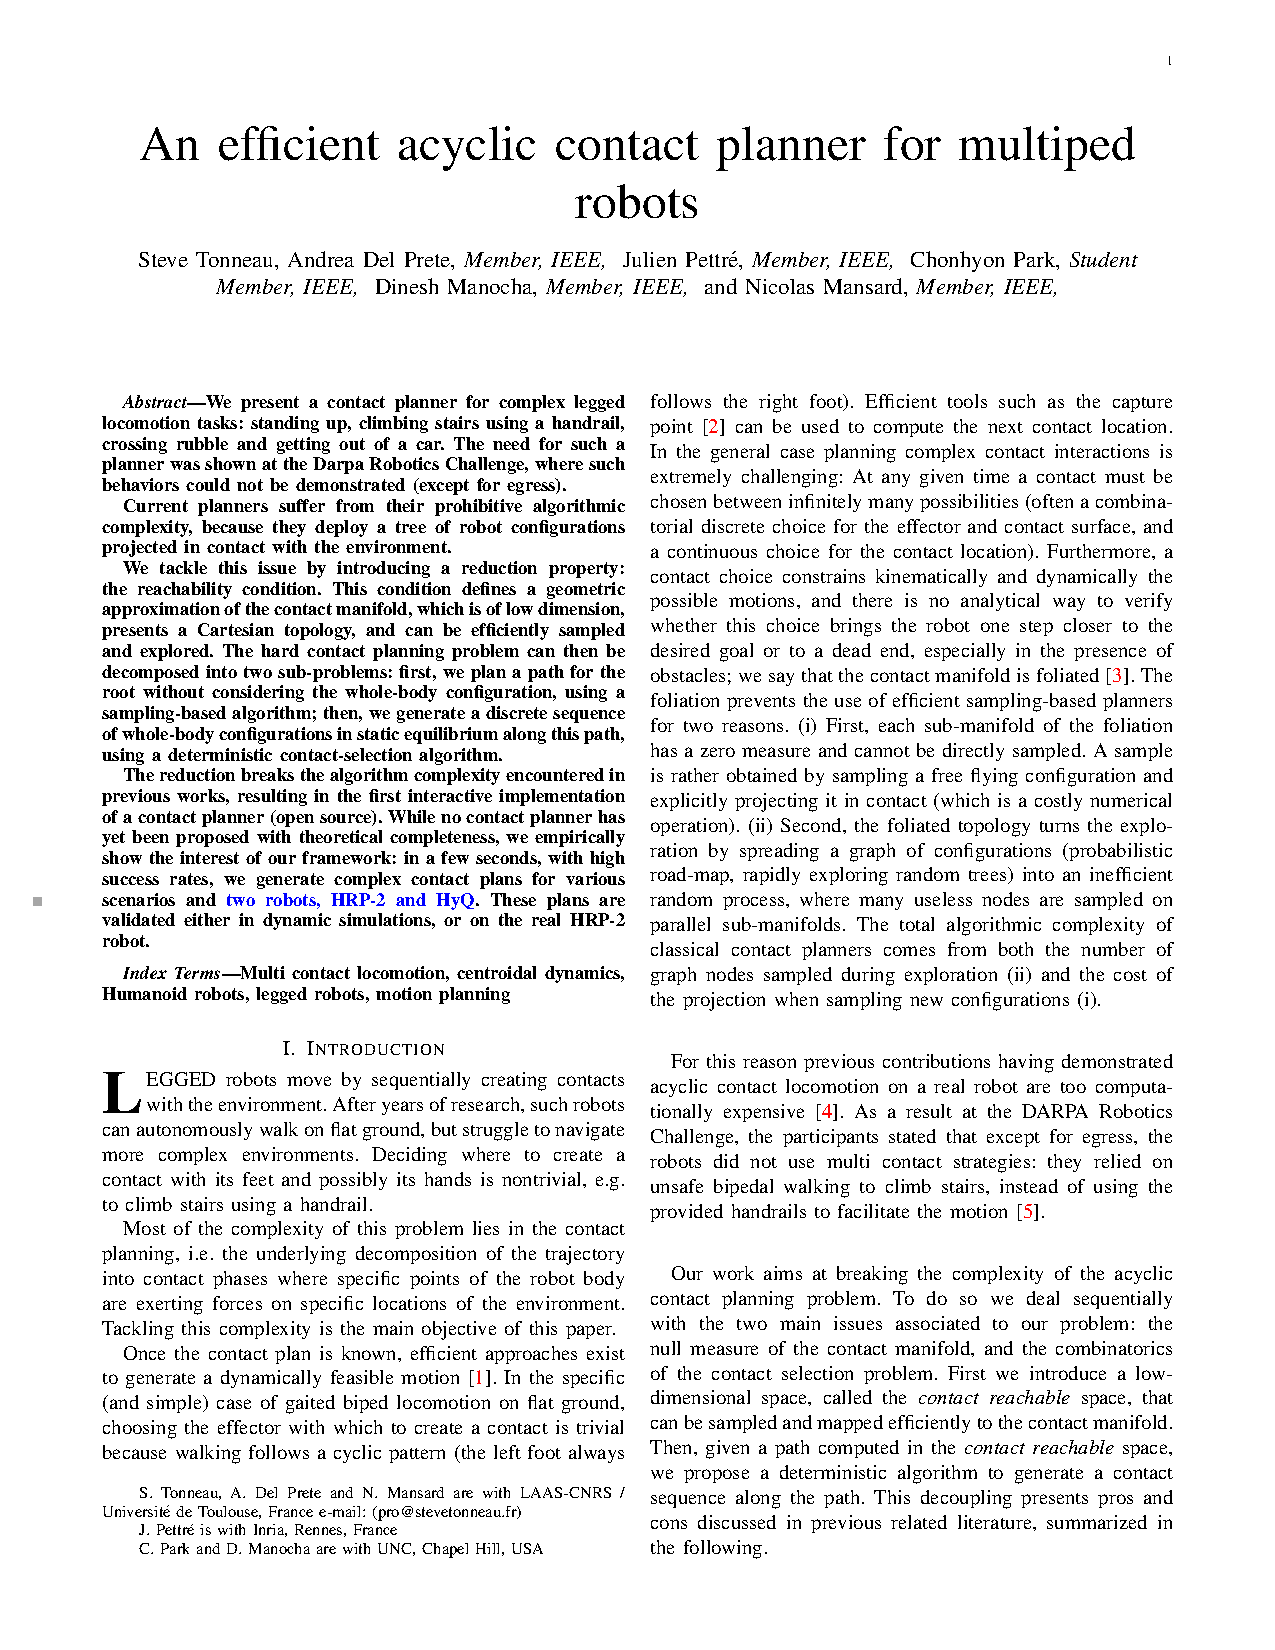
\includepdf[pages={-}]{diff.pdf}

\end{document}
